\begin{figure}[ht]
\centering
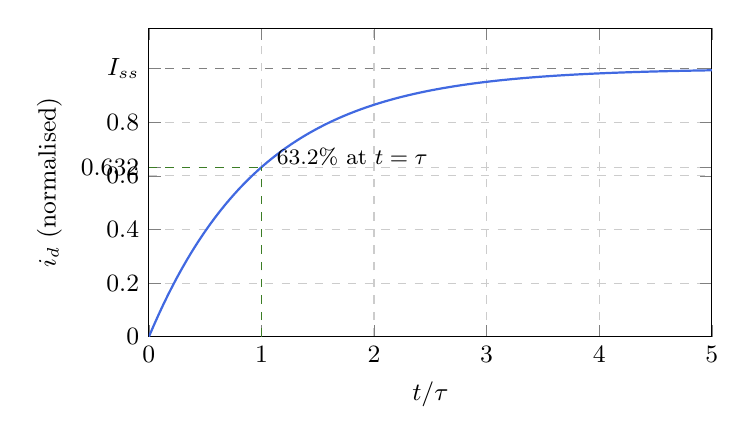
\begin{tikzpicture}
\begin{axis}[
  width=0.72\textwidth, height=5.5cm,
  xlabel={$t/\tau$}, ylabel={$i_d$ (normalised)},
  xmin=0, xmax=5, ymin=0, ymax=1.15,
  xtick={0,1,2,3,4,5},
  ytick={0,0.2,0.4,0.6,0.632,0.8,1.0},
  yticklabels={0,0.2,0.4,0.6,0.632,0.8,$I_{ss}$},
  grid=major, grid style={dashed,gray!40},
  tick label style={font=\small}, label style={font=\small},
]
\addplot[thick, RoyalBlue, domain=0:5, samples=120] {1 - exp(-x)};
\addplot[dashed, gray, domain=0:5] {1.0};
\addplot[dashed, OliveGreen, domain=0:1] {0.632};
\addplot[dashed, OliveGreen] coordinates {(1,0) (1,0.632)};
\node[font=\footnotesize, anchor=south west] at (axis cs:1.05,0.60)
  {$63.2\%$ at $t=\tau$};
\end{axis}
\end{tikzpicture}
\caption{DC step response: $i_d = I_{ss}(1 - e^{-t/\tau})$.
  $I_{ss} = V_{step}/R_{terminal}$. The $\tau$ crossing is marked but
  not used by the v2 estimator.}
\label{fig:dc-step-response}
\end{figure}
